\documentclass[preview]{standalone}
\usepackage{amsmath}
\usepackage{amssymb}
\usepackage{stellar}
\usepackage{definitions}
\usepackage{bettelini}
\usepackage{tikz}
\usepackage{pgfplots}
\pgfplotsset{compat=1.18}
\begin{document}
\id{diffeq-systems-initial-data}
\genpage
\section{Systems and initial data}

\begin{snippetdefinition}{diffeq-vector-cauchy-definition}{Vector initial value problem}
    Let \(\Omega\subseteq\realnumbers\times\realnumbers^m\) be open,
    \(f\colon\Omega\fromto\realnumbers^m\) continuous, and \((t_0,y_0)\in\Omega\).
    The \emph{initial value problem} is \(y'=f(t,y)\), \(y(t_0)=y_0\).
    A solution on an interval \(I\) containing \(t_0\) is a differentiable
    \function \(y\colon I\fromto\realnumbers^m\) with graph in \(\Omega\)
    satisfying these identities. It is automatically \(C^1\).
    On a closed interval, derivatives at its endpoints are understood one-sided.
\end{snippetdefinition}

\begin{snippetdefinition}{diffeq-boundary-value-definition}{Boundary and mixed data}
    For \(y^{(k)}=f(t,y,\ldots,y^{(k-1)})\), a \emph{boundary value problem}
    imposes conditions at distinct points, for example \(y(t_i)=v_i\),
    \(1\leq i\leq k\). A \emph{mixed problem} may prescribe both values and
    derivatives at different points. A Cauchy problem instead prescribes
    all \(y^{(j)}(t_0)\), \(0\leq j<k\), at a single point.
\end{snippetdefinition}

\begin{snippetnote}{diffeq-data-local-global}{Local and global questions}
    Initial data describe a local question near one point. Conditions at
    several points require a solution spanning those points; merely prescribing
    the expected number of conditions does not guarantee existence or uniqueness.
    The domain of a solution lies in the component of the time projection of
    \(\Omega\) containing its initial time, but it may be smaller because of
    escape to the boundary or finite-time blow-up.
\end{snippetnote}

\begin{snippetdefinition}{diffeq-well-posed-definition}{Well-posed problem}
    Relative to specified spaces and topologies for data and solutions,
    a differential-equation problem is \emph{well posed} if its solution exists,
    is unique and depends continuously on the data.
    The data may include initial values and the right-hand side.
    A problem failing any of these requirements is \emph{ill posed}.
\end{snippetdefinition}

\begin{snippetproposition}{diffeq-higher-order-system-reduction}{Reduction to a first-order system}
    Let \(f\) be continuous on an open subset of
    \(\realnumbers\times(\realnumbers^m)^k\).
    The equation \(y^{(k)}=f(t,y,\ldots,y^{(k-1)})\) is equivalent to
    \[
        Y_1'=Y_2,\ \ldots,\ Y_{k-1}'=Y_k,\qquad
        Y_k'=f(t,Y_1,\ldots,Y_k),
    \]
    with \(Y=(y,y',\ldots,y^{(k-1)})\in\realnumbers^{mk}\).
    Initial derivatives become the components of \(Y(t_0)\).
\end{snippetproposition}

\begin{snippetproof}{diffeq-higher-order-system-reduction-proof}{diffeq-higher-order-system-reduction}{Reduction to a first-order system}
    If \(y\in C^k(I,\realnumbers^m)\) solves the higher-order equation,
    differentiating the components gives the system and \(Y\in C^1\).
    Conversely, a \(C^1\) solution \(Y\) satisfies successively
    \(Y_2=Y_1',\ldots,Y_k=Y_1^{(k-1)}\). The last equation implies
    \(Y_1\in C^k\) and the original equation. The initial conditions correspond
    component by component. Thus first-order vector equations suffice for the general theory.
\end{snippetproof}

\section{Integral curves and singular branches}

\begin{snippetdefinition}{diffeq-geometric-integral-curve}{Geometric integral curve}
    For a planar relation \(M(x,y)\,dx+N(x,y)\,dy=0\),
    a \emph{regular integral curve} is a \(C^1\) parametrized curve
    \(\gamma(s)=(x(s),y(s))\), with \(\gamma'(s)\neq0\), satisfying
    \[
        M(\gamma(s))x'(s)+N(\gamma(s))y'(s)=0.
    \]
    Where \(x'\neq0\) and \(N\neq0\), it is locally the graph of a
    classical solution of \(dy/dx=-M/N\). The geometric relation may also
    admit vertical tangents where this explicit equation does not apply.
\end{snippetdefinition}

\begin{snippetexample}{diffeq-vertical-tangent-example}{A vertical tangent}
    The graph \(y=\sqrt[3]x\) satisfies \(y'=1/(3x^{2/3})\) for \(x\neq0\),
    but is not a classical solution at zero. Its full curve has the regular
    parametrization \(\gamma(s)=(s^3,s)\), and is the graph \(x=y^3\)
    in reversed coordinates. It satisfies \(dx-3y^2\,dy=0\) even at the origin.
\end{snippetexample}

\begin{snippetexample}{diffeq-cubic-gluing-example}{Envelopes do not list all solutions}
    The translated cubics \(y=(x-c)^3\) solve \(y'=3y^{2/3}\), with the real
    cube root. Their envelope \(y=0\) also solves the equation.
    More generally, for \(a\leq b\),
    \[
        y(x)=\begin{cases}(x-a)^3,&x<a,\\0,&a\leq x\leq b,\\(x-b)^3,&x>b\end{cases}
    \]
    is a \(C^1\) solution; either nonzero branch may be omitted.
    Thus the cubics and their envelope alone are not the general solution.
    Local uniqueness holds where \(y\neq0\), but fails at every
    \((x,0)\), including the zero point of a cubic.
\begin{center}
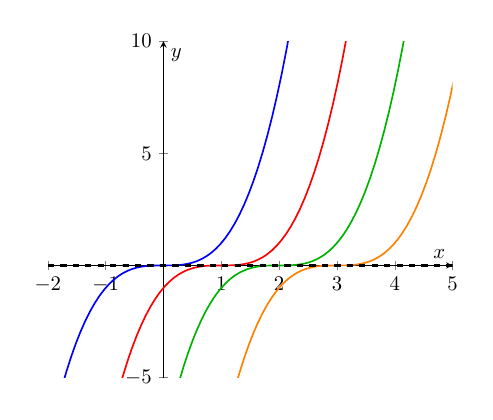
\begin{tikzpicture}[scale=0.75]
                \begin{axis}[
                        axis lines = middle,
                        xlabel = \(x\),
                        ylabel = \(y\),
                        xmin=-2, xmax=5,
                        ymin=-5, ymax=10,
                        domain=-2:6,
                        samples=100,
                        restrict y to domain=-10:15,
                    ]
                    \addplot[blue, thick] {(x-0)^3};
                    \addplot[red, thick] {(x-1)^3};
                    \addplot[green!70!black, thick] {(x-2)^3};
                    \addplot[orange, thick] {(x-3)^3};
                    \addplot[black, ultra thick, dashed, domain=-2:6] {0};
                \end{axis}
            \end{tikzpicture}
\end{center}
\end{snippetexample}

\begin{snippetnote}{diffeq-envelope-caution}{Checking a singular solution}
    A regular envelope of a one-parameter family can yield a singular solution,
    but tangency alone is not enough: it must satisfy the differential relation.
    Even then, additional joined solutions may exist when uniqueness fails.
\end{snippetnote}

\end{document}
